\documentclass[a4paper, 12pt]{article}

\usepackage[margin=25mm]{geometry}

\usepackage{hyperref}

\usepackage{graphicx}
\usepackage{svg}

\usepackage{amsmath}
\usepackage{amsfonts}
\usepackage{amssymb}

\usepackage{verbatim}

\usepackage{titlesec}

\usepackage{indentfirst}

\usepackage{csquotes}

\usepackage{enumitem}

\usepackage[nounderscore]{syntax}

\usepackage{caption}

\usepackage[ukrainian, english]{babel}

\usepackage{fontspec}
\setmainfont{CMU Serif}
\setsansfont{CMU Sans Serif}
\setmonofont{CMU Typewriter Text}

\usepackage{etoolbox}
\patchcmd{\thebibliography}{\section*{\refname}}{}{}{}

\title{Automatic solving of physics word problems}
\author{Ruslan Popov, Nadiia Karpenko \\
	\small Oles Honchar Dnipro National University (Ukraine)}

\date{}

\providecommand{\keywords}[1]
{
	\small	
	\textbf{\textit{Keywords---}} #1.
}

\newcommand{\etext}[1]{\enquote{\textit{#1}}}

\setlength{\grammarparsep}{0pt}

\setlength{\belowcaptionskip}{-10pt}

\setlength\parindent{24pt}

\makeatletter
\renewcommand*{\@seccntformat}[1]{\csname the#1\endcsname.\hspace{5pt}}
\makeatother

\renewcommand{\labelenumii}{\theenumii}
\renewcommand{\theenumii}{\theenumi.\arabic{enumii}.}

\begin{document}
	\maketitle
	
	\begin{abstract}
		We present a system that solves simple physics
		word problems (PWPs) stated in the English language. PWP is an
		interesting subfield of word problems that is not studied as deeply as
		math word problems (MWPs). We described the process of analyzing English
		text, the representation of problems, and algorithms for finding the
		solution. We have researched the types of PWPs and described their
		problem-solving strategies. We have noted the peculiarities that PWPs
		introduce in comparison to MWPs. We discussed the capabilities and
		limitations of our implementation and proposed future research areas.
	\end{abstract}
	
	
	\keywords{physics word problems, automatic problem
	solving, artificial intelligence, natural language processing, natural
	language understanding.}
	
	\section{INTRODUCTION}
	
	With the publication of Large Language Models (LLMs), students are
	tempted to solve their school problems by using AIs such as ChatGPT,
	Bard, etc. However, recent studies show that LLMs cannot solve physics
	problems well \cite{frust_soc}. Indeed, LLMs are neural models that try to
	predict the next word of the answer probabilistically. Thus, neither
	students nor engineers can trust the output of the model.
	
	Solving word problems is a classic and challenging field of AI
	programming. The automatic solving of such problems involves natural
	language processing, a well-formed problem representation, and a good
	problem-solving strategy.
	
	In this paper, we want to study the automatic solving of physics word
	problems.
	
	There are several reasons for the relevance of our paper:
	
	\begin{itemize}
	\item
	  The field of word problem solving is very diverse, and its research
	  has not developed as quickly as the research, for example, of neural
	  networks.
	\item
	  A significant research gap exists in understanding how to solve word
	  problems within specific scientific fields (such as physics,
	  chemistry, etc.) , whereas MWP solving has been a well-established
	  area of study.
	\item
	  Physics word problems bring new challenges in automatic solving that
	  require specific techniques to overcome them.
	\item
	  While many arithmetic word problem data sets exist, there is no widely
	  used collection of physics problems.
	\end{itemize}
	
	We want to revive the classic AI approach where programs solve human
	problems in a correct and deterministic way, where programs utilize the
	field knowledge, rules, and definitions to give a strict and accurate
	answer.
	
	\section{LITERATURE ANALYSIS}
	
	\subsection{STUDENT: Pioneer AI program}
	
	The D. Bobrow's STUDENT program is one of the first AI programs to
	understand natural language, showing promising results \cite{student}. The
	program solves algebraic word problems stated in English. An example of
	the problem that STUDENT can handle:
	
	\etext{If the number of customers Tom gets is twice the square of 20\%
	of the number of advertisements he runs, and the number of
	advertisements is 45, then what is the number of customers Tom gets?}''
	
	The STUDENT approach is straightforward: the problem is represented as a
	set of simultaneous equations; the solution of the problem is the
	solution for that set. The program used pattern matching and kernel
	sentence theory to transform English text into a set of equations. For
	the example above, STUDENT would generate this system:
	
	$$
	\begin{cases}
		(CUSTOMERS) = 2 * (0.2 + (ADVERTISMENTS)) ^ 2 \\
		
		(ADVERTISMENTS) = 45 \\
		
		? = (CUSTOMERS)
	\end{cases}
	$$
	
	Words in the problem text resemble mathematical operations and
	variables, so the STUDENT can translate the English text into
	mathematical expressions using pattern matching. The question mark is a
	special symbol used to denote the unknown value. The variables in the
	equation are subparts of the problem text.
	
	When the set of equations is unsolvable, the STUDENT will try to solve
	it again with several techniques applied. For example, STUDENT may
	change variable names to be equal if they have some words in common
	(e.g., \etext{SPEED} and \etext{SPEED OF THE CAR}). Or, the
	STUDENT may add new equations from its internal knowledge of the world.
	
	The STUDENT program is nearly 60 years old. The field of AI programming
	has improved since that time. Peter Norvig presented an analysis and
	elegant implementation of STUDENT written in Common Lisp in functional
	programming style \cite{paip}.
	
	\subsection{Math word problem solvers}
	
	We want to continue the literature overview by analyzing math word
	problem solvers. We want to inherit the researched knowledge of natural
	language processing and problem representation that is studied in this
	field of word problem-solving.
	
	Here is the list and analysis of different problem representations for
	MWPs structured by Mandal et al. \cite{mwp_repr}:
	
	\begin{itemize}
	\item
	  Equation template representation. An equation template is a
	  predetermined equation that is formed with arithmetic operations and
	  with two types of unknowns (called slots): unknown variables and
	  numbers. Using statistical approaches, the words in the problem are
	  aligned into these unknown slots.
	\item
	  Equation tree representation. The whole problem is converted into an
	  equation tree using statistical methods. Usually, recognizers generate
	  several trees, so another approach is applied to choose the best.
	\item
	  Entity and state transition-based representation. In this approach,
	  the problem consists of states and state transitions. A state contains
	  all the information of the known objects (their owners, count, and
	  type). State transition would change the count of belonging objects,
	  which can result in an equation.
	\item
	  Tag-based representation. In this method, the text is processed in
	  several stages. First, it is tokenized and parsed. Then, the type of
	  problem is recognized. After that, several logic forms representing
	  grammatical relations and quantities are generated. An answer is
	  generated using special techniques.
	\end{itemize}
	
	The natural language processing of MWPs has many methods, including
	rule-based techniques and statistical and neural models. Often, solvers
	parse the English text into dependency trees. Common features extracted
	from the text are part of speech tag, the lemma of a word, quantities,
	units of quantities, comparative adverbs, dependencies between verbs and
	quantities, etc. \cite{mwp_nlp}.
	
	\subsection{Physics word problem solvers}
	
	There is not so much research and categorization on PWP solvers. Most
	programs date back to 1970-1980 and use their own knowledge
	representation and custom natural language processing methods.
	
	One of the first programs that could handle PWP is the NEWTON program by
	Kleer \cite{newton}. It is made to solve mechanical problems. NEWTON would
	analyze the program\textquotesingle s text and convert it to several
	data structures. The first data structure depicts objects, and the
	second is a tree-like data structure (called \enquote{envisioning tree}) that
	holds all possible states of the objects. The tree\textquotesingle s
	root is the starting position, and the next children are the next
	events. When the tree divides, it means that there are several
	possibilities where an object could move. Quantitative knowledge is
	presented in a data structure called FRAME. It stores all the known
	parameters of the object and the equations that connect those
	parameters.
	
	Gordon S. Novak Jr. has studied the topic of physics problems very
	thoroughly. One of the programs he developed is ISAAC \cite{isaac}. This
	problem understands and solves physics problems that involve rigid
	bodies in static equilibrium. The program can also draw a diagram of the
	problem.
	
	ISAAC problem analysis consists of lots of stages, and they have several
	branches. Firstly, an augmented transition network transforms the
	English text into structured parsed sentences. Then, the semantic
	analysis is performed. It is used to determine the meaning of verbs and
	prepositions. After several stages, a canonical object model is formed.
	In this data structure, objects in the problem are represented as
	physics objects (point, pivot, lever, etc.). The canonical object model
	is then passed to the EUCLID program, which analyzes the orientation of
	objects and assigns coordinates to them. After that, the geometric model
	is formed. Problem-solving involves creating a set of equations that
	represent physical laws between objects.
	
	The ISAAC program is big and complex. It is hard to analyze it because
	of its age and programming style. As the author states, 44 pages of Lisp
	code is written only for parsing the English text, while problem-solving
	is one of the simplest parts of the program. We were unable to find the
	source code of the ISAAC program.
	
	Bundy et al. created the MECHO program, which addresses mechanical PWPs
	and is implemented in Prolog \cite{mecho}. The program processes the word
	problem in several stages. First, it parses the text, extracting
	information. Then, MECHO derives assertions related to objects, given
	parameters, and unknown values from the parsed data. These assertions
	are then transformed into a particular data structure called schema,
	where inference rules, resembling logical representations of physics
	laws in Prolog, are applied. MECHO can provide either symbolic or
	numerical solutions.
	
	Mukherjee et al. have an extensive overview of rule-based word problem
	solvers and a dedicated section for PWPs. Other programs for solving
	PWPs include BEATRIX, ALBERT, and FREEBODY \cite{other_pwp}. All those programs
	address only specific types of physics problems. As the reader may
	notice, all the names of the programs resemble human names and are
	written in upper-case. Possibly, this tradition came after the STUDENT
	program.
	
	We have found a modern paper on PWP solving. Leszczynski et al. address
	the problems of a free-falling object under constant acceleration of
	gravity \cite{modern_pwp}. The problem is analyzed using several recurrent neural
	networks (RNN), then the dynamical system is formed, and the solution is
	provided at the end. The first RNN is a word labeler used to extract the
	given values and the problem question. The second RNN is a classifier
	that determines the type of question. While this work seems modern and
	interesting, the accepted problem set is limited and generated
	artificially using context-free grammar.
	
	\subsection{Conclusions of literature analysis}
	
	We have investigated the design of several word problem solvers.
	Unfortunately, we concluded that a few techniques apply to make a
	generic PWP solver. Or at least the known methods cannot solve problems
	from Ukrainian physics textbooks.
	
	There are some issues in using STUDENT to solve physics problems.
	Consider the problem: \etext{If the distance between Dnipro and Kyiv is
	477 kilometers and the time the automobile has traveled is 6 hours, then
	what is the speed of the automobile?}. The STUDENT would generate this
	set of equations:
	
	$$
	\begin{cases}
		(DISTANCE) = 477\ kilometers \\
		
		(TIME) = 6\ hours \\
		
		? = (SPEED)
	\end{cases}
	$$
	
	As the reader may notice, the STUDENT has generated a system consisting
	of given values and unknowns. This set would resemble the column
	\enquote{Given}, which is usually written by students. But the physics problem
	cannot be represented like this set of equations for two reasons:
	
	\begin{enumerate}[label=\arabic*)]
	\item
	  This set is unsolvable. A set of equations requires that all the
	  information needed to find the unknowns is present in the set. But our
	  example has no connection between speed, time, and distance.
	\item
	  There is a theoretical issue. In math, variables represent unknown
	  values and act like bound variables in lambda calculus: their names
	  can be changed freely unless they interfere with another name. But in
	  the physics field, the name of variables has a special meaning. It is
	  a given value that marks some parameter of an object.
	\end{enumerate}
	
	In this example, STUDENT would add needed equations from its internal
	knowledge using the search on the first word of a variable (it may find
	the relation \etext{the distance is equal to time multiplied by
	speed}). While this approach may work for simple problems like the one
	above, it is not the best solution because it is too chaotic and
	brute-force-like.
	
	The approaches presented in subsection 2.2 are not sufficient to
	represent physics problems. They are constructed around math
	expressions, though in PWP, usually there are no explicitly stated
	expressions (only given values are specified).
	
	Most papers for word problem-solving are outdated. They use
	unstandardized programming languages with undefined styles of
	programming. The analysis of the capabilities and limitations of
	previous works is not enough.
	
	\section{OBJECT, SUBJECT, AND METHODS OF RESEARCH}
	
	\subsection{Object and subject}
	
	The object of our research is automatic word problem-solving. The
	subject of our research is the automatic solving of physics word
	problems.
	
	\subsection{Method of the research}
	
	To study the subject, we developed a program that can solve basic PWPs
	stated in the English language, which do not involve any dynamic change
	or complex representation. Also, we do not support solving problems
	where a graphical model is needed (forces, impulses, energy, etc.).
	
	The whole program was written in Python language. We have separated our
	program into two projects: one is a user interface, and the other is the
	core library. The technology stack of the user interface consists of
	Django (web framework), MathJax (LATEX output), and Bootstrap (graphical
	design). The library uses spaCy (natural language processing) and SymPy
	(symbolic math) libraries. We used PythonAnywhere to host our program
	(\url{https://inanyan.pythonanywhere.com/}).
	
	By definitions provided in AI:MA \cite{aima}, we consider our program to be
	inside the \enquote{Thinking Rationally} field because we are trying to find
	the computational model behind PWP solving and provide the user with a
	correct problem solution.
	
	The whole NLP pipeline, algorithms, and data structures that are used by
	our program can be depicted through this diagram:
	
	\begin{figure}[h]
		\centering
		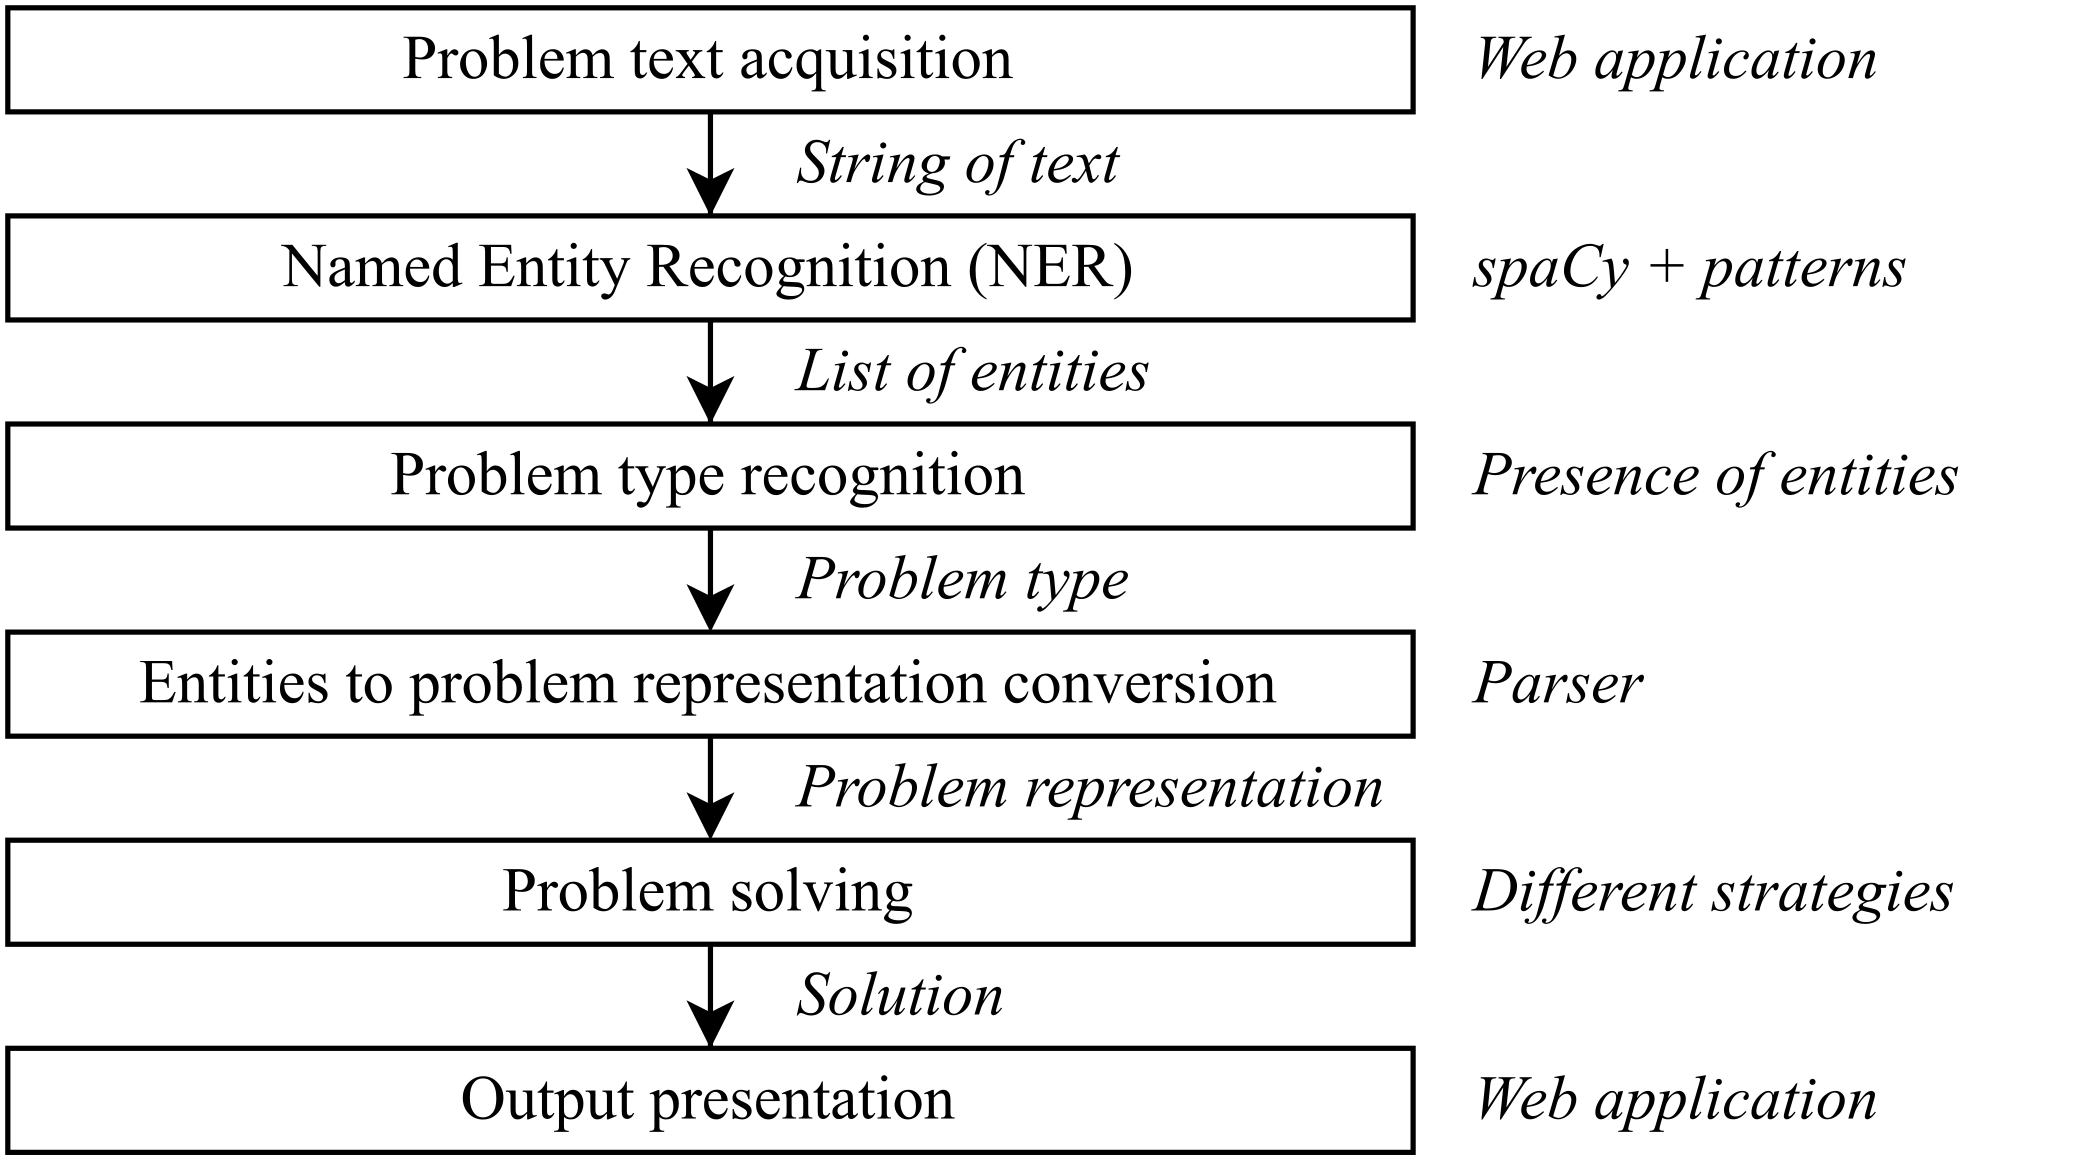
\includegraphics[width=0.75\textwidth]{media/image2.png}
		\caption{Algorithms and data structures of our program.}
	\end{figure}
	
	In fig. 1 nodes represent algorithms, right after the node comes a brief
	comment on the chosen approach, and the labels of the arrows are data
	structures. In section IV of the paper, we will describe all the steps
	of the program, but before that, we will discuss the found types of
	physics problems to understand what features we need to extract from
	English text.
	
	\subsection{Testing data}
	
	To test our program, we created a small dataset with physics problems
	collected from various sources such as \cite{ukr_ph_1}, \cite{ukr_ph_2}, and the
	Internet. We translated the Ukrainian variants to English.
	
	\section{DESCRIPTION OF THE PROGRAM}
	
	\subsection{Problem types}
	
	The first thing we did before starting to make this program was to study
	available PWP. We noticed that PWPs fall into five categories:
	
	\begin{itemize}
	\item
	  Theoretical problem: \etext{Why do we not observe the daily rotation
	  of the earth in everyday life?}.
	\item
	  Value conversion problem: \etext{The car is traveling at a speed of
	  108 kilometers per hour. Represent this speed in meters per second}.
	\item
	  Value comparison problem: \etext{Which speed is bigger: 10 meters per
	  second or 10 kilometers per hour?}.
	\item
	  Unknowns finding problem: \etext{The car drove for 40 minutes at a
	  speed of 144 kilometers per hour. How far did the car travel?}.
	\item
	  Calculation of the change of a value depending on other value changes:
	  \etext{How many times will the speed of wave propagation increase if
	  the wavelength increases by three times and the period of oscillation
	  remains unchanged?}.
	\end{itemize}
	
	We decided not to solve the theoretical problems because they require an
	extensive ontology of physics definitions and laws, while we were more
	focused on computational problems.
	
	\subsection{Named Entity Recognition}
	
	We chose the named entity recognition (NER) method for the feature
	extraction task. In this method, subparts of text, called entities, are
	marked with a particular string that represents the type of an entity.
	
	We have collected the information about which entities our program
	should recognize:
	
	\begin{itemize}
	\item
	  Given values: \etext{the distance is 10 kilometers}, \etext{the
	  mass is 50 grams}, etc.
	\item
	  Unknown values: \etext{What is the speed\ldots{}},
	  \etext{Determine the density of\ldots{}}, etc.
	\item
	  Units: \etext{meters per second}, \etext{kilogram}, \etext{Newton}, etc.
	\item
	  Value changes: \etext{time is increased by a factor of 2}, etc.
	\end{itemize}
	
	For NER, we chose a rule-based method -- pattern matching. We will
	present the patterns we used for NER with our modified BNF notation
	because there is no standardized way to do this. In this notation, no
	recursion is allowed. Terminals are written as is and may resemble
	either the lowercase form of a token or its lemma. Non-terminals are
	written inside `\textless' and `\textgreater'. Entities are written as
	non-terminals whose names are written in uppercase form; the other
	non-terminals are fragments used only for easier construction of the
	grammar. The special rule \textless like\_num\textgreater{} denotes one
	token resembling a number. An ellipsis indicates a part of the rule that
	was shortened in the paper.
	
	Here is the list of all the rules:
	
	\begin{grammar}
		\centering 
		
		<unit\_name> ::= meter | hour | kilogram | candela | lux | ...
		
		<modifier> ::= cubic | square
		
		<single\_unit> ::= [<modifier>] <unit\_name>
		
		<compound\_unit> ::= <single\_unit> per <single\_unit>
		
		<UNIT> ::= <single\_unit> | <compound\_unit>
		
		<QUANTITY> ::= <like\_num> <UNIT>
		
		<COMPARISON\_WORD> ::= greater | faster | bigger | larger | slower | less | ...
		
		<single\_term> ::= density | volume | speed | length | moment | force | ... 
		
		<compound\_term> ::= ampere force | wave propagation | ... 
		
		<simple\_term> ::= <single\_term> | <compound\_term> 
		
		<of\_term> ::= <simple\_term> of [<determiner>] <simple\_term> 
		
		<TERM> ::= <simple_term> | <of_term>
		
		<UNKNOWN\_QUESTION> ::= what | determine | calculate
		
		<special\_unknown\_word> ::= far | fast | often
		
		<UNKNOWN\_HOW\_QUESTION> ::= how <special\_unknown\_word>
		
		<neg\_change\_word> ::= decrease | reduce
		
		<pos\_change\_word> ::= increase
		
		<determiner> ::= a | an | the
		
		<change\_pattern> ::= by [<determiner> factor of] <like_num>
		
		<NEG\_CHANGE> ::= <neg\_change\_word> <change\_pattern>
		
		<POS\_CHANGE> ::= <pos\_change\_word> <change\_pattern>
		
		<CHANGE\_VERB> ::= <pos\_change\_word> | <neg\_change\_word> | change
		
	\end{grammar}
	
	We provide here an example of NER to understand this process better:
	
	\begin{figure}[h]
		\centering
		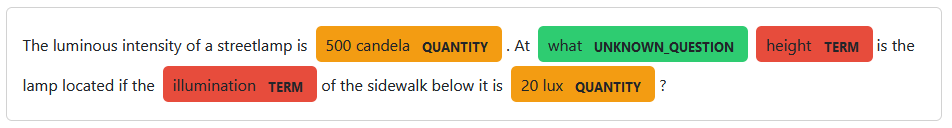
\includegraphics[width=\textwidth]{media/image3.png}
		\caption{Example of named entity recognition for an unknown finding problem.}
	\end{figure}
	
	\begin{figure}[h]
		\centering
		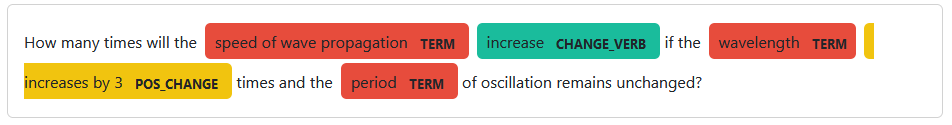
\includegraphics[width=\textwidth]{media/image4.png}
		\caption{Example of named entity recognition for a value change problem.}
	\end{figure}
	
	\subsection{Problem type recognition}
	
	The program determines the type of problem by looking at the presence of
	entities. The algorithm can be described in English like this:
	
	\begin{enumerate}
	\item
	  If there is a CHANGE\_VERB entity, then it is a value change problem.
	\item
	  If there is a UNIT entity, then it is a conversion problem.
	\item
	  If there is a COMPARSON\_WORD entity, then it is a comparison problem.
	\item
	  If there is an UNKNOWN\_QUESTION or UNKNOWN\_HOW\_QUESTION entity,
	  then it is an unknown finding problem.
	\item
	  Otherwise, the program cannot recognize the type of problem.
	\end{enumerate}
	
	\subsection{Entities to problem representation conversion}
	
	The algorithm for converting a list of entities to problem
	representation according to the recognized problem type can be described
	like this:
	
	\begin{enumerate}
	\item
	  For value conversion problem, extract a quantity and a unit.
	\item
	  For value comparison problems, extract two quantities.
	\item
	  For unknowns finding problem, extract given and unknown values.
	\item
	  For value change problems, extract the value changes and the value in
	  question.
	\end{enumerate}
	
	To convert a quantity into the internal math representation, the program
	converts the number (the first token) and the unit (the rest).
	
	We have found that units in SymPy are written as regular English words,
	allowing us to use Python's insecure \enquote{eval} function. The program will
	convert the unit entity into a valid Python expression and call the
	\enquote{eval} function. We replace the word \etext{per} with the division
	symbol. To parse the modifiers \etext{square} and \etext{cube}, we
	replace those words with \enquote{**2} and \enquote{**3}, respectively, after the
	single unit.
	
	We have found two ways in which given values are encoded in the list of
	entities. It is either a pair of TERM and QUANTITY or a single QUANTITY.
	
	To convert the pair of TERM and QUANTITY into a given value, the program
	needs to convert the term into a symbol (the QUANTITY will be the value
	of a given variable). The program uses a hard-coded map data structure,
	the key to which is a string, and the value is a symbol (e.g.,
	\etext{force} is \(F\), \etext{mass} is \(m\), etc.).
	
	A special technique for determining the symbol should be applied to
	convert a single QUANTITY into a given value. We have found that looking
	at the unit of a quantity can infer the variable. If the unit is one
	English word, the program uses a hard-coded map data structure (e.g.,
	\etext{meters} is \(S\), \etext{seconds} is \(t\), etc.).
	
	The conversion of compound units and units with modifiers is tricky.
	However, we noticed that compound units resemble a physical formula
	(e.g., \etext{meters per second} corresponds to \(v = \frac{S}{t}\),
	etc.). So, the program will first convert all one-word units in the
	compound unit to the symbols. Then, if the expression is not a single
	unit, the program will search the list of formulas for a formula, the
	right-hand side of which is identical to the result expression.
	
	The whole process described above ended up being so powerful that the
	program will use it while presenting the output of value comparison and
	conversion problems.
	
	Unknown values are encoded either as a pair of UNKNOWN\_QUESTION and
	TERM or as a single UNKNOWN\_HOW\_QUESTION. For the first variant, it is
	sufficient to convert the TERM into a variable, and for the second
	variant, we use a hard-coded map data structure (e.g., \etext{how
	far} is \(S\), \etext{how fast} is \(\upsilon\), etc.).
	
	Value changes are encoded as a pair of TERM and POS\_CHANGE or TERM and
	NEG\_CHANGE. To convert these pairs into a variable change, the program
	should infer the variable by the TERM entity and determine the factor of
	the variable change. According to our NER rules, the factor number comes
	at the end of the POS\_CHANGE and NEG\_CHANGE. So, it is enough to parse
	the last token in the span. If the entity is NEG\_CHANGE, the parser
	should also take the number\textquotesingle s reciprocal.
	
	The value under change is encoded as a pair of TERM and CHANGE\_WORD. It
	is enough to infer the variable from the TERM entity.
	
	\subsection{Problem-solving}
	
	Solving value conversion and comparison problems is trivial, and it is a
	primitive operation in the SymPy library, so we will not describe these
	processes. However, we note that for value comparison problems, the
	program will convert the second value to the unit of the first value.
	
	We define the solution to unknowns finding problems as a list of
	formulas. This list resembles a plan of actions that the computer should
	perform. The calculation of the final answer is delegated to the output
	part of our program.
	
	The first attempt to solve an unknown finding problem would be to use a
	search algorithm for each unknown variable to find a formula left-hand
	side of which is equal to the unknown. But this approach is wrong for
	several reasons:
	
	\begin{itemize}
	\item
	  The program could find several applicable formulas for one unknown.
	\item
	  The formula may contain an unknown variable (a variable that is not
	  given). However, it is possible to find another formula that could be
	  used to find those variables.
	\item
	  One physical formula can be used to find several variables. Consider
	  the second Newton's law: \(F = ma\). This formula can be used not only
	  to find a force but also a mass (if the force and the acceleration are
	  known) or an acceleration (if the force and the mass are known).
	\end{itemize}
	
	These discussions guided us to make this recursive algorithm:
	
	\begin{enumerate}
	\item
	  Find an applicable formula for the unknown variable.
	\item
	  Create a set difference of given variables and the free symbols in the
	  found formula. This set will resemble the set of unknowns of a
	  formula.
	\item
	  If the set is empty, return a list of one element containing the found
	  formula (base case).
	\item
	  Otherwise, perform these steps:
	
	  \begin{enumerate}
	  \item
	    For each element in the set, apply this algorithm (recursive step).
	  \item
	    Combine all the results. The final result is a list.
	  \item
	    Append the found formula to the list.
	  \item
	    Return the list.
	  \end{enumerate}
	\end{enumerate}
	
	We described this algorithm informally because the algorithm can fail in
	several steps. If the algorithm fails on step 1 or step 4.1, this may
	mean two things: the program cannot find the solution for the unknown
	variable in the problem representation, or the program should find
	another formula to apply.
	
	Also, we used the term \enquote{applicable formula}. This means the formula
	belongs to the internal list of formulas or is derived.
	
	We have quickly noticed that this algorithm is a simplified version of
	the Stanford Research Institute Problem Solver algorithm \cite{strips}. So,
	we modified it to the physical field. The goals are represented as math
	symbols. The operators are the applicable formulas. The preconditions of
	an operator (or a formula) are the free symbols of the formula. The
	initial step is represented as a set of given.
	
	We define the solution to a value change problem as an ordered pair of a
	floating-point number and a formula. The number is the result of
	dividing the value of a changed value and the original value, and the
	formula is used to present the output for the user.
	
	We invented this problem-solving algorithm for this problem type:
	
	\begin{enumerate}
	\item
	  Find a formula for which the given variables are a subset of the
	  formula's variables.
	\item
	  Substitute each formula variable with the given variables as a
	  \enquote{factor * variable}.
	\item
	  Divide the derived formula with the original formula.
	\item
	  If the result is a number, then it is the answer to the problem.
	\item
	  Otherwise, repeat from step \#1 and find another formula.
	\end{enumerate}
	
	The algorithm may fail at step 1 or 5, meaning the program could not
	find the formula to calculate the change. The algorithm is simple, and
	it resembles human thinking.
	
	\subsection{Context}
	
	The first time we made a prototype of the program, we noticed it was
	limited. Consider a problem: \etext{What is the optical power of a
	converging lens with a focal length of 40 centimeters?}. A special
	formula solves this problem (\(D = \pm \frac{1}{F}\)). However, the
	formula varies whether the lens is a converging lens or a diverging
	lens. Another situation when we find this peculiarity is when we need to
	calculate the surface of an object (squares, rectangles, triangles,
	etc.).
	
	We introduce the term context to encode the information about a physical
	object. Context is a set of strings that encode objects and their
	qualities. Examples of context words: \etext{lens},
	\etext{converging}, \etext{diverging}, \etext{square},
	\etext{cube}, \etext{rectangle}, etc. In each physics problem,
	there is an associated context.
	
	\section{RESULTS}
	
	\subsection{Examples of program usage}
	
	We will present the solution of 4 problems with different types and
	comment on how the program solved them.
	
	Problem \#1: \etext{The car is traveling at a speed of 108 kilometers
	per hour. Represent this speed in meters per second}.
	
	\begin{figure}[h]
		\centering
		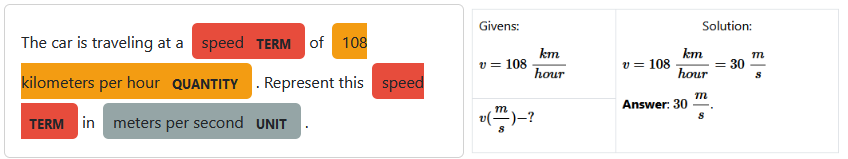
\includegraphics[width=\textwidth]{media/image5.png}
		\caption{The program results for problem \#1.}
	\end{figure}
	
	Problem \#1 is a conversion problem. We haven't found many problems of
	this type. The program correctly recognized the given quantity and
	target unit. There is no detailed explanation of the solution because
	conversion is a primitive operation in SymPy.
	
	Problem \#2: \etext{Which speed is slower: 72 kilometers per hour or 24
	meters per second?}.
	
	\begin{figure}[h]
		\centering
		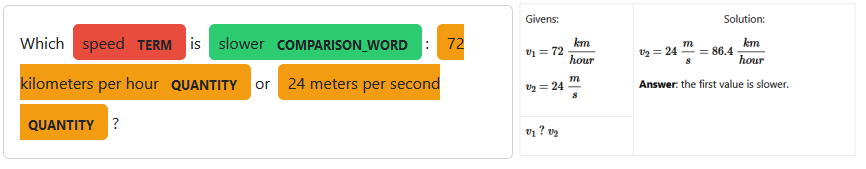
\includegraphics[width=\textwidth]{media/image6.png}
		\caption{The program results for problem \#2.}
	\end{figure}
	
	Problem \#2 is a comparison problem. It is not trivial to compare
	\(72\frac{km}{h}\) and \(24\frac{m}{s}\). The program correctly
	recognized two quantities and the type of the problem. According to our
	problem-solving strategy, the program converted the second value to the
	unit of the first value. Also, our program generates answers based on
	the word that was asked. For example, if the question asks for greater
	value, the answer will show greater value, and in this example, the
	program tells us about slower value.
	
	Problem \#3: \etext{To raise a marble column weighing 3.78 tons from
	the bottom of a lake, 95200 joules of work was done. Determine the depth
	of the lake}.
	
	\begin{figure}[h]
		\centering
		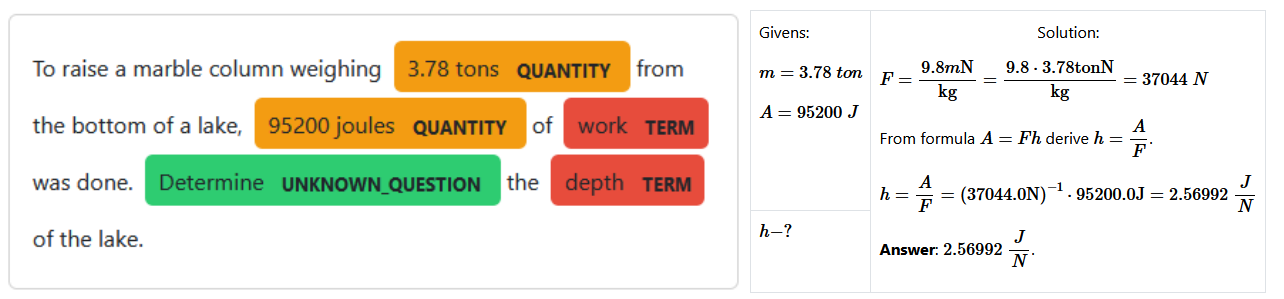
\includegraphics[width=\textwidth]{media/image7.png}
		\caption{The program result for problem \#3.}
	\end{figure}
	
	Problem \#3 is an unknown finding problem. We chose this problem because
	it is not so trivial to solve; it includes several formulas for the
	solution. Unfortunately, this example shows some peculiarities of SymPy
	and our implementation, which we will discuss in the following
	subsection.
	
	The program correctly recognized the given variables and the unknown
	variable. The program correctly found the solution, including the
	gravitational force and work formulas. Additionally, the program derived
	the height from the work formula.
	
	Problem \#4: \etext{How many times will the moment of a force change if
	the force is increased by a factor of 8 and the arm of the force is
	decreased by a factor of 4?}.
	
	\begin{figure}[h]
		\centering
		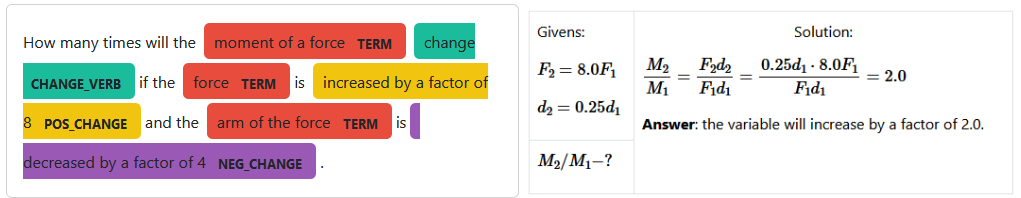
\includegraphics[width=\textwidth]{media/image8.png}
		\caption{The program results for problem \#4.}
	\end{figure}
	
	Problem \#4 is a value change problem. A parser is needed to convert the
	list of entities to the problem representation fully. The program
	correctly recognized the given changes and the value under question. The
	program found the required formula and performed a substitution, which
	resulted in a number.
	
	Special attention is required to the term entities. We included the
	preposition \etext{of} in the term. Usually, while recognizing noun
	phrases (NP), different NPs stay away, but we combined them and
	determined the variable based on the first words. If we did not make
	this decision, an ambiguity would arise: do we need to find the change
	of the moment or the force?
	
	\subsection{Analysis of limitations of the program}
	
	We performed a thorough analysis of issues that our program has. We
	grouped the issues into several categories:
	
	\begin{enumerate}
	\item
	  Complex problem types.
	\item
	  Imperfect natural language processing.
	\item
	  Inaccurate problem type recognition.
	\item
	  Incomplete problem representation.
	\item
	  Imperfect problem-solving techniques.
	\item
	  Symbol is semantically equal to terms and objects.
	\item
	  Issues with libraries that we use.
	\end{enumerate}
	
	We want to begin the analysis of the limitations of our program by
	analyzing our problem-type classification. We have found that our types
	can have new subtypes. Consider the problem: \etext{Can a wedding ring
	with a volume of 0.5 cubic centimeters and a mass of 8 grams really be
	gold?}. It is a new question type for which the answer is a Boolean
	value. But it is easy to notice that this is a subtype of unknown
	finding problem. The program must compare the object's density to the
	actual gold density.
	
	There are lots of issues with natural language processing. We have found
	that the solution to the problem depends highly on the problem
	formulation. A possible reason is that we used a rule-based approach for
	NER. Rule-based techniques are usually used on the first iteration of
	NLP program development, and then they are replaced by more powerful
	statistical or neural models \cite{nlp}.
	
	Pattern matching, used for NER, restricts the input text to a specific
	syntax. For example, we require that the units are written as proper
	English words instead of their abbreviations. The program cannot
	recognize numbers that are not written with decimal notation (e.g.,
	\etext{one second}). The patterns require that every quantity has a
	corresponding unit (the program cannot parse \etext{1 and 4
	kilograms} as two quantities). Change of a value should be written as
	\etext{increased by 9} or \etext{reduced by a factor of 2} (but
	the program cannot parse \etext{the value is halved} or
	\etext{doubled}). There are many ways to formulate the problem, so
	there could be lots of patterns in the text that the programmer may
	miss.
	
	Another interesting problem that our application has is that it cannot
	support tasks with named constants. The program cannot infer that the
	\etext{length of the equator} is about \(4 \cdot 10^{4}\, km\). Also
	consider the problem: \etext{Find the volume of mercury weighing 2
	kilograms}. The program needs to refer to the table of densities and
	update the problem representation. Our implementation does not do it.
	
	The most interesting issue with parsing English text is that it is easy
	to deceive the program. Consider the problem: \etext{The airplane flew
	1200 kilometers in 2 hours. At what speed did the airplane fly?}. The
	program can handle it. But if the user adds this sentence to the end of
	the text: \etext{Represent the result in meters per second}, then our
	implementation will think that this problem is a value conversion
	problem. So, looking at keywords is not the best approach to determine
	the type of problem.
	
	Our problem representation is too basic. The physics problem is not a
	set of given variables and unknowns. An image or a diagram may be
	included, but the program cannot analyze them. An equation may be
	offered.
	
	However, one of the biggest issues with problem representation is that
	we do not support several objects in the task. The program cannot
	recognize the two velocities of two bodies or two
	capacitors\textquotesingle{} capacitance values in an electric chain.
	The problem lies in the representation of variables; we use only one
	symbol for them, but an index could also be used in the real world.
	
	The solution to some problem types may be more complicated than we
	provide. This can be illustrated by this problem: \etext{The masses of
	two steel balls are 1 kilogram and 4 kilograms. Which of the balls has
	the greater volume? By how many times?}. Again, it is a simple problem
	for a human to solve, but not the computer. Our program would think this
	is a comparison problem and happily answer that 4 kilograms is bigger
	than 1. The program should use a formula for inferring the volume of
	objects, but our implementation handles only the given quantities.
	
	Our problem-solving strategy for value change problems is imperfect. We
	defined that the answer to a value change problem results from division.
	But we can compare values not only with division but also with
	subtraction. Also, we implicitly assume that the physical formulas are
	created with multiplication and division of variables so that the
	variables will be reduced in the division step. But if the formula is
	formed with addition, then this strategy will not work.
	
	Consider the problem: \etext{How would the mass of an iron ball change
	if its radius is increased by a factor of two?}. This problem requires
	two formulas to find (one for the volume and one that involves the
	density of iron). It is easy to notice that we can reuse the STRIPS
	algorithm to find the unknowns of the first formula, but there lies a
	new degree of complexity.
	
	We propose a hypothesis that it is impossible to construct an efficient
	algorithm for solving value change problems. For every unknown variable
	in the formula, the program should decide whether to leave it as is
	(hoping it will be reduced in the division) or to find another formula.
	But that second formula could also have unknown variables. Moreover, it
	may miss some changes if the program doesn't use a formula for some
	unknowns.
	
	There is a theoretical issue with our program. Our problem-solving
	algorithm treats physical terms and objects as variables. But, in the
	real world, variables resemble physical terms. With this issue, an
	ambiguity arises: \(c\) may mean either capacitance or speed of light,
	but the program considers these terms equal because they are written
	with the same symbol.
	
	We have used a special technique for treating a QUANTITY entity as a
	given value if there is no TERM entity. If the program encounters a
	\etext{2 meters}'' entity, it will treat it as \(S = 2\ m\). We have
	found that this is another ambiguity in our implementation. This entity
	can be not only \(S\), but also \(l\), \(h\), \(d\), etc.
	
	There are also various issues with the libraries we use. The SymPy
	treats the unit of a physical value as a variable, so problems with
	printing may arise. Another problem is that SymPy does not know that
	Joule divided by Newton is a meter. Not enough units are provided in the
	SymPy library. The library documentation is too short, and we have not
	found a simple way to resolve these issues.
	
	\section{CONCLUSIONS}
	
	In this paper, we have studied the automatic solving of physics word
	problems. PWP solving is a challenging subfield of word problem solving
	that requires complex problem representation. We have found that
	researched solutions for math word problems are unsuitable for solving
	PWP. Current PWP solvers are focused on specific problem types, while we
	were interested in generic PWP solvers.
	
	To study our paper\textquotesingle s object and subject, we developed
	and described a program that could solve simple physics problems. Our
	testing dataset was formed from Ukrainian physics textbooks. The
	development of word problem solvers focuses mainly on problem
	representation, natural language processing, and problem-solving
	strategies.
	
	Our analysis shows that PWPs fall into five categories: theoretical,
	value conversion, value comparison, unknowns finding, and value change
	problems.
	
	To convert problem text into the internal problem representation, we
	chose named entity recognition based on pattern matching. Other
	techniques for NER besides pattern matching on tokens can be used to
	analyze problem text, such as pattern matching on trees and statistical
	and neural models. Problem types are recognized based on the presence of
	particular entities. While this approach was sufficient on our small
	dataset, we have noticed that this solution could be easily broken.
	After NER, another step is required to convert a list of entities into
	the representation.
	
	We have found a new kind of ambiguity: \enquote{quantity without a term}. This
	type of ambiguity occurs when the program finds a quantity entity that
	is a given value, but the program cannot infer the variable for this
	quantity. We partially solved this problem by inferring the variable by
	the unit of the quantity.
	
	Our research shows that the algorithm for solving problems with unknown
	values is the STRIPS algorithm. Value change problems are complex
	problems to solve because of many non-trivial parameters. We hypothesize
	that these problems cannot be solved efficiently and belong to the class
	of \enquote{NP-hard} problems.
	
	While our program can solve static computational physics problems, it is
	obvious that there are many other types of physics problems. Our program
	can be improved by choosing different NLP methods and by developing a
	more sophisticated problem representation.
	
	\section{REFERENCES}
	
	\bibliographystyle{apalike}
	\bibliography{lit}
\end{document}